\section{Yarrawonga and Mulwala: Demand-Responsive Transportation in Regional Victoria, Australia}
\label{sec:yarrawonga}
\hfill \textbf{Author:} Nicole Ronald

\editdone{This text has undergone the professional edit. Please no grammatical changes anymore! They are most-probably wrong.}

% ==================================================================================================================
In November 2013, Public Transport Victoria (PTV) implemented a service called
Flexiride in twin regional Victoria towns, consisting of an on-demand public
transport service using taxis. This service replaced an existing fixed-route bus
service, which was poorly patronized.
%\ah{I replace PTV everywhere by its full name as PTV is so prominent with VISUM}

This scenario was designed to investigate operational performance change  
 between two different \gls{drt} schemes: Flexiride and a
completely ad-hoc scheme. More details can be found in
\citep[][]{RonThoWin2015}. This work was a first step in developing a
decision-support tool to evaluate different \gls{drt} schemes, particularly when
integrated with other transport modes. 

% --------
%Associated projects: 
The scenario was part of a larger project exploring the viability of
mobility-on-demand, focusing on ridesharing and \gls{drt} services \citep[][]{Ronald_iMoD_2014}.

% --------
%Study area: 
The scenario covered twin towns on the border of Victoria and New South Wales,
Australia, separated by the Murray River. Yarrawonga (Victoria) has a population
of 7\,057 and an area of 95.0\,square kilometers, while Mulwala (New South Wales) has a
population of 1\,904 and an area of 18.6\,square kilometers. 

The Flexiride scheme delivered six services on weekdays and three services on
Saturday, leaving Yarrawonga center (Orr St) at fixed times. The local
taxi operator was paid a holding fee by Public Transport Victoria to have a taxi available at
Orr St at the nominated time. The taxi returned to normal service when there were no
bookings or passengers waiting.

Passengers could ride either by phone booking, at least 10\,minutes before
the service was scheduled to depart from Orr St, or by arriving at Orr St in
person to begin their trip. Existing bus stops were used as pickup and drop-off
points.

Figure~\ref{fig:yarrawonga} shows the stops in both towns; the main stop in Yarrawonga, Orr St, is denoted by a star.
%
\createfigure%
{Location of bus stops in Yarrawonga/Mulwala}%
{Location of bus stops in Yarrawonga/Mulwala, including \gls{od} zones}%
{\label{fig:yarrawonga}}%
{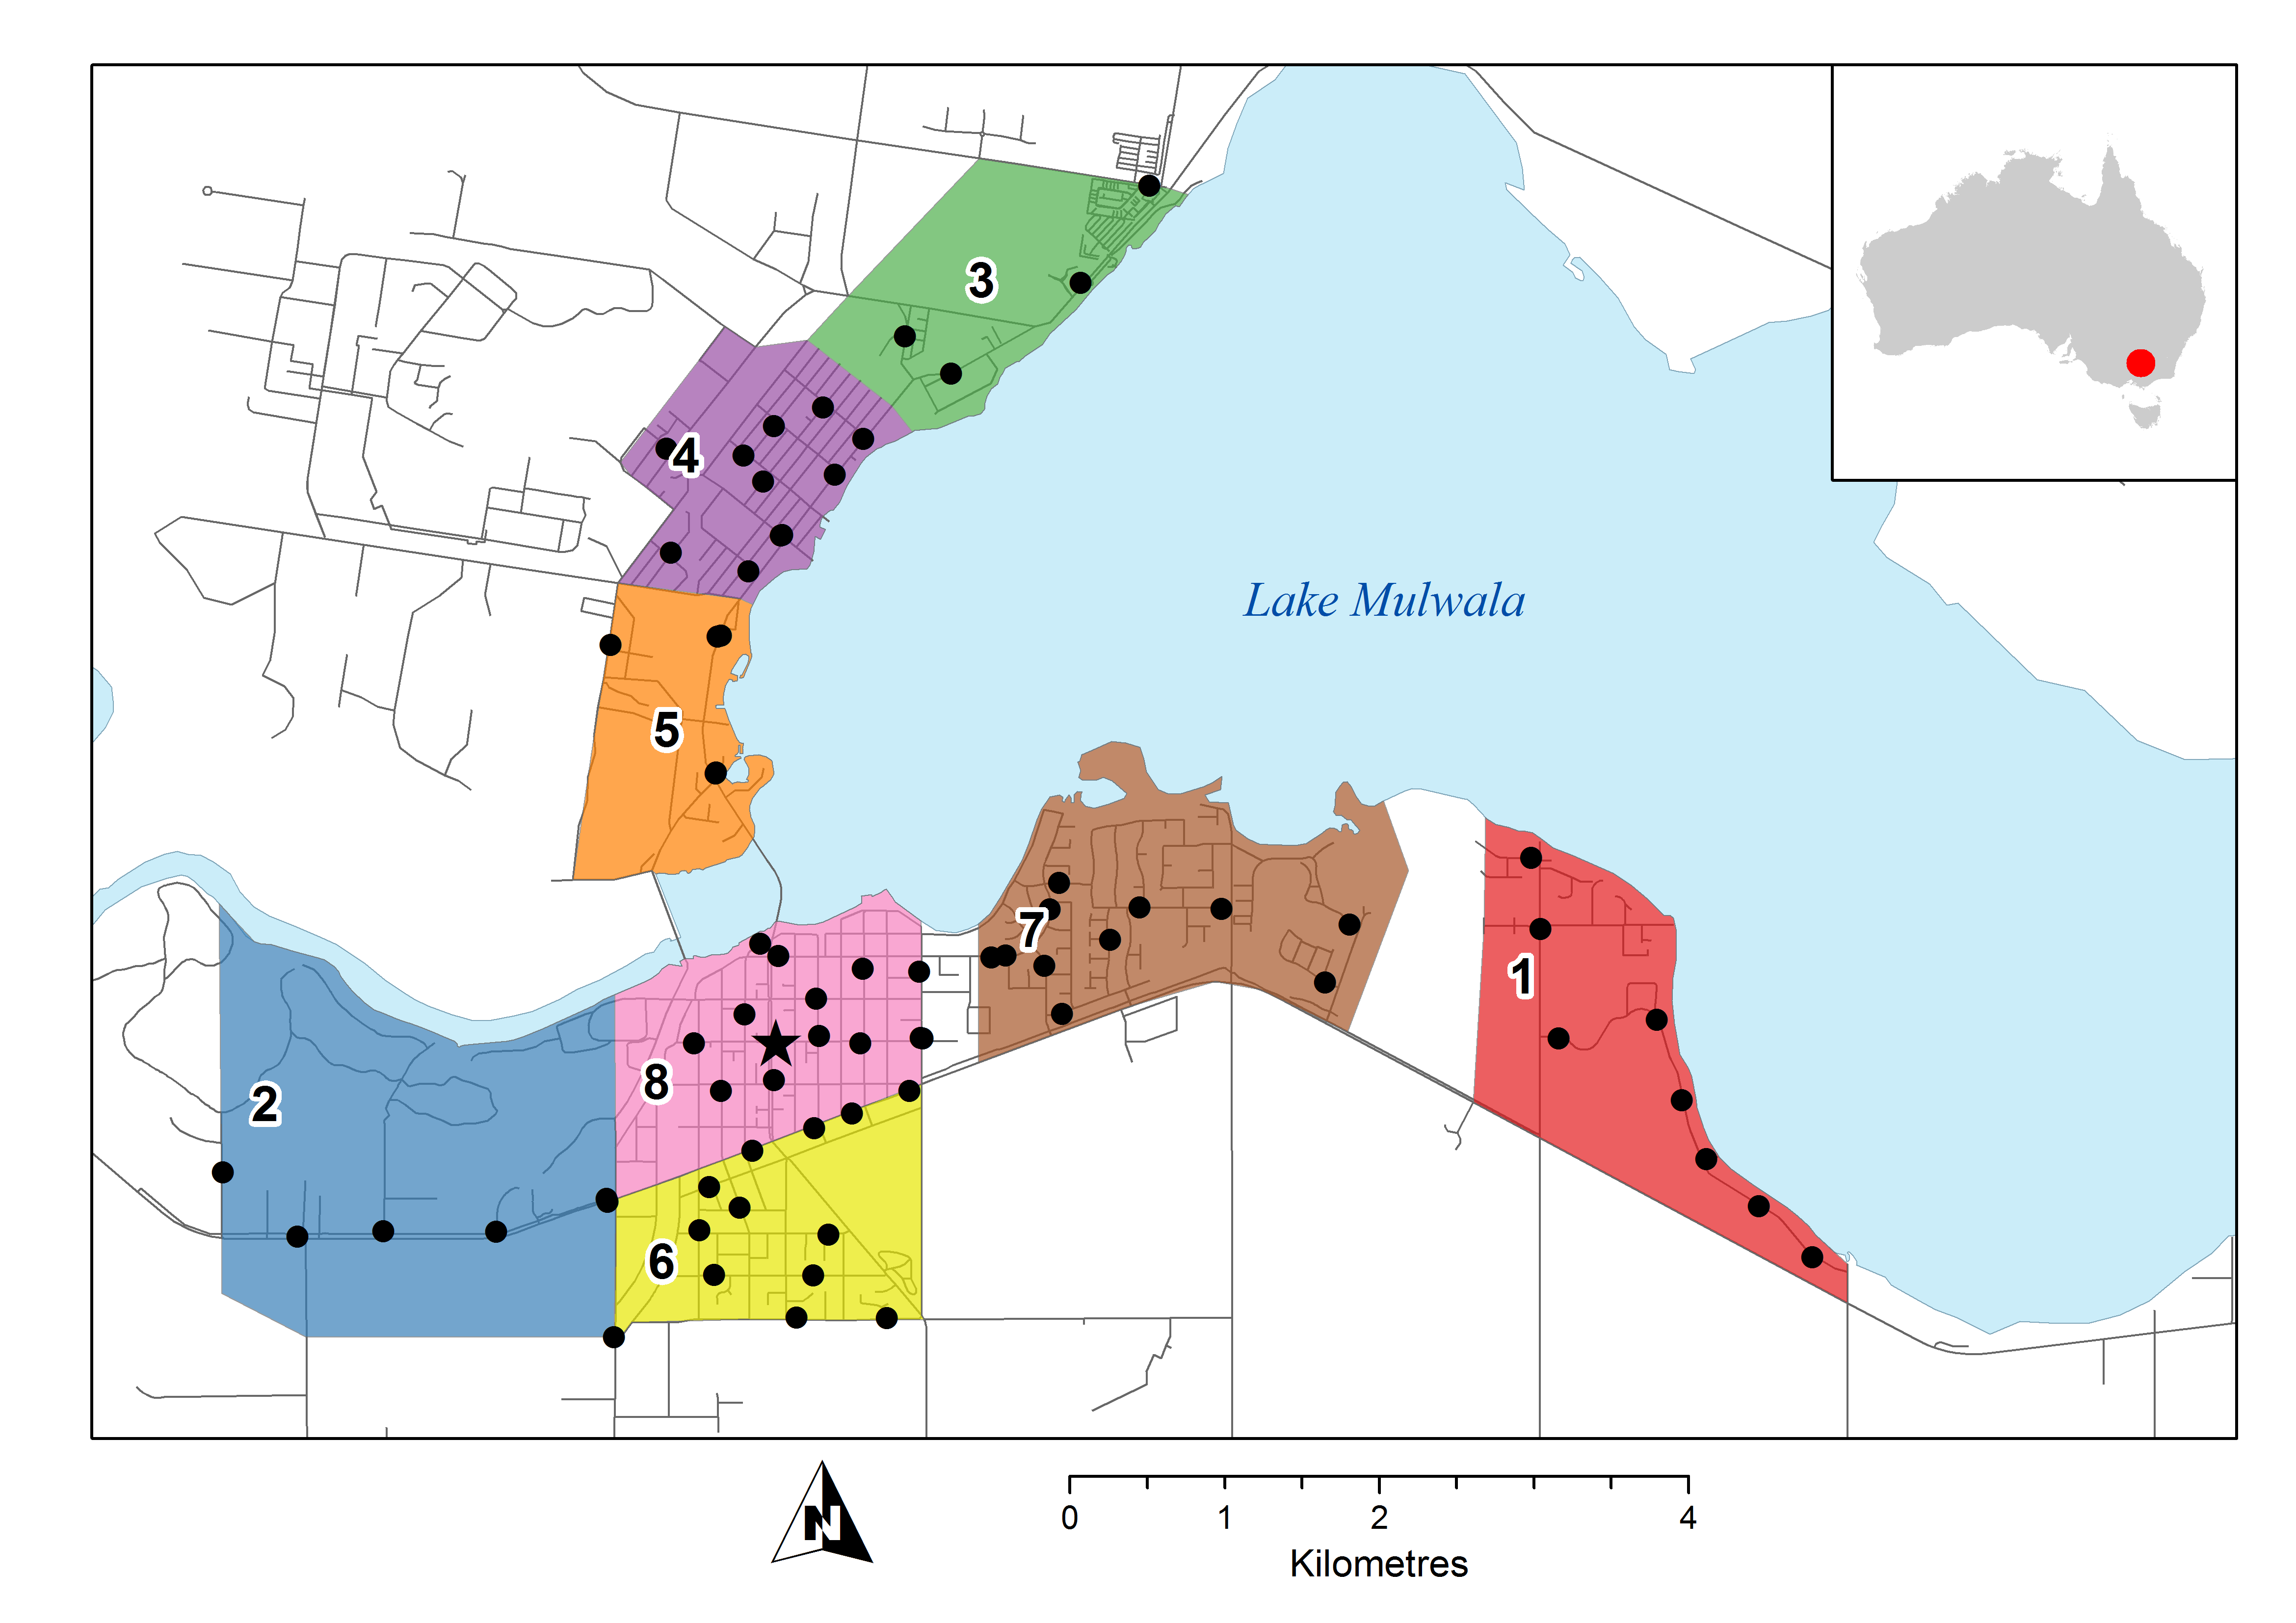
\includegraphics[width=0.85\textwidth, angle=0]{./using/figures/yarrawonga_high.png}}%
{}
%
% --------

Flexiride drivers recorded pickup locations and drop-offs for each service,
as well as fare revenue collected. Using this data, probabilities of trips
occurring between two zones were developed, using the process in
\citet[][]{Deflorio_ITSIET_2011}. A continuous departure time distribution was
derived from evenly spreading demand for particular services to either side
of that service. 

% --------
%Activity Locations: not used

% --------
%Network:
The network was extracted from \gls{osm}. Some bus stops were removed if they were assigned to the same link in \gls{matsim}, \eg stops on the same road between intersections.

% --------
%Modes:
Only passengers for the demand-responsive service were included. However, the use of \gls{matsim} for this initial model means that other modes could be added in later versions.

% --------
%Calibration and validation: exploratory

% --------
%Simulation quality and achieved results:
This was an exploratory simulation that demonstrated how \gls{drt} could be modeled for exploring viability and comparison of different schemes.

Using \gls{matsim}, experimentation with varying demands, two different scheduling
algorithms and an altered Flexiride service, with more services, were
carried out. Outcomes like drive time, vehicle-kilometers traveled and
passenger wait time could be measured.

Results showed that the two schemes performed differently for operators and
passengers. Optimization schemes had little effect in low demand situations, while
seating requirements showed more variability in the ad-hoc scheme, as demand
increased. Future work involves estimating  both schemes' costs for further
comparison.

This work was supported by a grant from the Australian Research Council (LP120200130). We are also grateful to Michal Maciejewski for his assistance with the \gls{dvrp} extension (see Chapter~\ref{ch:dts}). Michael Rigby prepared the map of Yarrawonga and Mulwala.
% ==================================================================================================================
